\documentclass[ignorenonframetext,]{beamer}
\setbeamertemplate{caption}[numbered]
\setbeamertemplate{caption label separator}{: }
\setbeamercolor{caption name}{fg=normal text.fg}
\beamertemplatenavigationsymbolsempty
\usepackage{lmodern}
\usepackage{amssymb,amsmath}
\usepackage{ifxetex,ifluatex}
\usepackage{fixltx2e} % provides \textsubscript
\ifnum 0\ifxetex 1\fi\ifluatex 1\fi=0 % if pdftex
\usepackage[T1]{fontenc}
\usepackage[utf8]{inputenc}
\else % if luatex or xelatex
\ifxetex
\usepackage{mathspec}
\else
\usepackage{fontspec}
\fi
\defaultfontfeatures{Ligatures=TeX,Scale=MatchLowercase}
\fi
% use upquote if available, for straight quotes in verbatim environments
\IfFileExists{upquote.sty}{\usepackage{upquote}}{}
% use microtype if available
\IfFileExists{microtype.sty}{%
\usepackage{microtype}
\UseMicrotypeSet[protrusion]{basicmath} % disable protrusion for tt fonts
}{}
\newif\ifbibliography
\usepackage{color}
\usepackage{fancyvrb}
\newcommand{\VerbBar}{|}
\newcommand{\VERB}{\Verb[commandchars=\\\{\}]}
\DefineVerbatimEnvironment{Highlighting}{Verbatim}{commandchars=\\\{\}}
% Add ',fontsize=\small' for more characters per line
\usepackage{framed}
\definecolor{shadecolor}{RGB}{248,248,248}
\newenvironment{Shaded}{\begin{snugshade}}{\end{snugshade}}
\newcommand{\KeywordTok}[1]{\textcolor[rgb]{0.13,0.29,0.53}{\textbf{{#1}}}}
\newcommand{\DataTypeTok}[1]{\textcolor[rgb]{0.13,0.29,0.53}{{#1}}}
\newcommand{\DecValTok}[1]{\textcolor[rgb]{0.00,0.00,0.81}{{#1}}}
\newcommand{\BaseNTok}[1]{\textcolor[rgb]{0.00,0.00,0.81}{{#1}}}
\newcommand{\FloatTok}[1]{\textcolor[rgb]{0.00,0.00,0.81}{{#1}}}
\newcommand{\ConstantTok}[1]{\textcolor[rgb]{0.00,0.00,0.00}{{#1}}}
\newcommand{\CharTok}[1]{\textcolor[rgb]{0.31,0.60,0.02}{{#1}}}
\newcommand{\SpecialCharTok}[1]{\textcolor[rgb]{0.00,0.00,0.00}{{#1}}}
\newcommand{\StringTok}[1]{\textcolor[rgb]{0.31,0.60,0.02}{{#1}}}
\newcommand{\VerbatimStringTok}[1]{\textcolor[rgb]{0.31,0.60,0.02}{{#1}}}
\newcommand{\SpecialStringTok}[1]{\textcolor[rgb]{0.31,0.60,0.02}{{#1}}}
\newcommand{\ImportTok}[1]{{#1}}
\newcommand{\CommentTok}[1]{\textcolor[rgb]{0.56,0.35,0.01}{\textit{{#1}}}}
\newcommand{\DocumentationTok}[1]{\textcolor[rgb]{0.56,0.35,0.01}{\textbf{\textit{{#1}}}}}
\newcommand{\AnnotationTok}[1]{\textcolor[rgb]{0.56,0.35,0.01}{\textbf{\textit{{#1}}}}}
\newcommand{\CommentVarTok}[1]{\textcolor[rgb]{0.56,0.35,0.01}{\textbf{\textit{{#1}}}}}
\newcommand{\OtherTok}[1]{\textcolor[rgb]{0.56,0.35,0.01}{{#1}}}
\newcommand{\FunctionTok}[1]{\textcolor[rgb]{0.00,0.00,0.00}{{#1}}}
\newcommand{\VariableTok}[1]{\textcolor[rgb]{0.00,0.00,0.00}{{#1}}}
\newcommand{\ControlFlowTok}[1]{\textcolor[rgb]{0.13,0.29,0.53}{\textbf{{#1}}}}
\newcommand{\OperatorTok}[1]{\textcolor[rgb]{0.81,0.36,0.00}{\textbf{{#1}}}}
\newcommand{\BuiltInTok}[1]{{#1}}
\newcommand{\ExtensionTok}[1]{{#1}}
\newcommand{\PreprocessorTok}[1]{\textcolor[rgb]{0.56,0.35,0.01}{\textit{{#1}}}}
\newcommand{\AttributeTok}[1]{\textcolor[rgb]{0.77,0.63,0.00}{{#1}}}
\newcommand{\RegionMarkerTok}[1]{{#1}}
\newcommand{\InformationTok}[1]{\textcolor[rgb]{0.56,0.35,0.01}{\textbf{\textit{{#1}}}}}
\newcommand{\WarningTok}[1]{\textcolor[rgb]{0.56,0.35,0.01}{\textbf{\textit{{#1}}}}}
\newcommand{\AlertTok}[1]{\textcolor[rgb]{0.94,0.16,0.16}{{#1}}}
\newcommand{\ErrorTok}[1]{\textcolor[rgb]{0.64,0.00,0.00}{\textbf{{#1}}}}
\newcommand{\NormalTok}[1]{{#1}}
\usepackage{longtable,booktabs}
\usepackage{caption}
% These lines are needed to make table captions work with longtable:
\makeatletter
\def\fnum@table{\tablename~\thetable}
\makeatother

% Prevent slide breaks in the middle of a paragraph:
\widowpenalties 1 10000
\raggedbottom

\AtBeginPart{
\let\insertpartnumber\relax
\let\partname\relax
\frame{\partpage}
}
\AtBeginSection{
\ifbibliography
\else
\let\insertsectionnumber\relax
\let\sectionname\relax
\frame{\sectionpage}
\fi
}
\AtBeginSubsection{
\let\insertsubsectionnumber\relax
\let\subsectionname\relax
\frame{\subsectionpage}
}

\setlength{\parindent}{0pt}
\setlength{\parskip}{6pt plus 2pt minus 1pt}
\setlength{\emergencystretch}{3em}  % prevent overfull lines
\providecommand{\tightlist}{%
\setlength{\itemsep}{0pt}\setlength{\parskip}{0pt}}
\setcounter{secnumdepth}{0}

\title{Risk analysis and Urban Planning and Development}
\subtitle{Real-Estate Investments - Tutorial 6}
\author{Or Levkovich}
\date{13 October 2017}

\begin{document}
\frame{\titlepage}

\begin{frame}{Urban Planning and Development}

Factors influencing on housing demand:

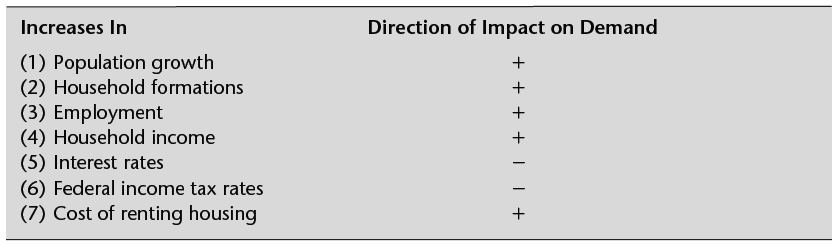
\includegraphics[width=300 px]{housing_demand}

\end{frame}

\begin{frame}{Risk analysis}

Changes in demand affect returns and increase investments risks.

Evaluating risk by examining the expected return:

\begin{itemize}
\tightlist
\item
  IRR under favourable and unfavourable scenarios.
\item
  Partitioning IRR to analyze risk factors.
\end{itemize}

\end{frame}

\begin{frame}{``Real options'' approach}

Reducing risk by not fully commiting to invest all capital at one point
in time.

\begin{itemize}
\tightlist
\item
  Developer can purchase a parcel of land, but keep the decision of when
  to construct (given current and expected market conditions).
\item
  Development project can also be partially constructed.
\end{itemize}

The developer can decide to wait for improved market conditions,
reducing investment risk. The lower risk is captured in the value of
land.\footnote<.->{see presentation slides}

\end{frame}

\begin{frame}{Land valuation under ``real options'' approach}

\normalsize

Land developed faces the option to develop her land today, or in one
year. She uses the real options approach to help decide when to
construct:

\begin{itemize}
\tightlist
\item
  Compute current value of land (using the residual method).
\item
  Consider that the land is developed, and the market may follow two
  scenarios: Optimistic and pessimistic (in which conditions are the
  same as today).
\end{itemize}

\end{frame}

\begin{frame}{Land valuation under ``real options'' approach
(continued)}

\normalsize

\begin{itemize}
\tightlist
\item
  Compare the scenarios with a situation in which the land was not
  developed, and instead the developer invested in a ``replicate''
  portfolio. The portfolio consists of \(\alpha\) housing units and
  \(\beta\) shares of risk free assets. \(\alpha\) and \(\beta\) are
  determined in a way that reflects the return for both scenarions.
\end{itemize}

\[ V = \alpha*P + \beta \] Where \(V\) is the value of land, \(P\) is
the price per constructed unit.

\begin{itemize}
\tightlist
\item
  Use \(\alpha\) and \(\beta\) to calculate the value of a replicate
  portfolio and compare it with current expected return (no
  construction). Use this value to support the decision of whether to
  build or not.
\end{itemize}

\end{frame}

\begin{frame}{Land valuation under ``real options'' approach (Example)}

Land value = units*(price - cost).

\begin{longtable}[]{@{}llllll@{}}
\toprule
Scenario & price & units & costs & Land value & Interest\tabularnewline
\midrule
\endhead
Current & 0.29M & 10 & 0.17M & 1.20M & 4\%\tabularnewline
Optimistic & 0.33M & 15 & 0.19M & 2.10M & 4\%\tabularnewline
Pessimistic & 0.28M & 10 & 0.18M & 1.00M & 4\%\tabularnewline
\bottomrule
\end{longtable}

\(2.1 = \alpha*0.33 + \beta*1.04\)

\(1.0 = \alpha*0.28 + \beta*1.04\)

\footnotesize
*Note: we assume that the risk-free shares paid interest during the
year*. \small

\(\alpha = 22\), \(\beta = -4.9615\)

\(V = 22*0.29 -4.9615 = 1.4185\)

1.4185M \(>\) 1.20M : Construction in one year is preferred.

\normalsize

\end{frame}

\section{Exercises}\label{exercises}

\begin{frame}{Problem 1 (p.~447)}

Two investments have the following pattern of expected returns:

\begin{center}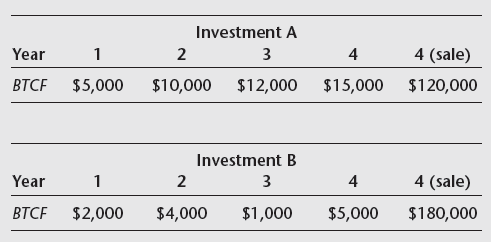
\includegraphics[width=200 px]{p1_447} \end{center}

Investment A requires an outlay of \$110,000 and Investment B requires
an outlay of \$120,000.

\begin{enumerate}
\def\labelenumi{\arabic{enumi}.}
\tightlist
\item
  What is the BTIRR on each investment?
\item
  If the BTIRR were partitioned based on BTCFo and BTCFs what
  proportions of the BTIRR would be represented by each?
\item
  What do these proportions mean?
\end{enumerate}

\end{frame}

\begin{frame}[fragile]{Problem 1 (p.447) Answers}

\footnotesize

\begin{Shaded}
\begin{Highlighting}[]
\CommentTok{# 1 }
\NormalTok{=}\KeywordTok{IRR}\NormalTok{(-}\DecValTok{110000}\NormalTok{,}\DecValTok{5000}\NormalTok{,}\DecValTok{10000}\NormalTok{,}\DecValTok{12000}\NormalTok{,}\DecValTok{15000}\NormalTok{,}\DecValTok{120000}\NormalTok{) }
\NormalTok{=}\StringTok{ }\FloatTok{9.2}\NormalTok

\CommentTok{# 2 }
\NormalTok{PV of operation }\KeywordTok{CF} \NormalTok{(A):}\StringTok{ }\DecValTok{32}\NormalTok{,}\FloatTok{727.1}
\NormalTok{PV of operation }\KeywordTok{CF} \NormalTok{(B):}\StringTok{ }\DecValTok{9}\NormalTok{,}\FloatTok{469.6}
\NormalTok{PV of sale }\KeywordTok{CF} \NormalTok{(A) :}\StringTok{ }\DecValTok{77}\NormalTok{,}\FloatTok{272.8}
\NormalTok{PV of sale }\KeywordTok{CF} \NormalTok{(B) :}\StringTok{ }\DecValTok{115}\NormalTok{,}\FloatTok{909.3}

\KeywordTok{BTIRRo} \NormalTok{(A) :}\StringTok{ }\DecValTok{32}\NormalTok{,}\FloatTok{727.1}\NormalTok{/(}\DecValTok{32}\NormalTok{,}\FloatTok{727.1}\DecValTok{+77}\NormalTok{,}\FloatTok{272.8}\NormalTok{) =}\StringTok{ }\FloatTok{29.75}\NormalTok

\KeywordTok{BTIRRo} \NormalTok{(B) :}\StringTok{ }\DecValTok{9}\NormalTok{,}\FloatTok{469.6}\NormalTok{/(}\DecValTok{9}\NormalTok{,}\FloatTok{469.6}\DecValTok{+115}\NormalTok{,}\FloatTok{909.3}\NormalTok{) =}\StringTok{ }\FloatTok{7.55}\NormalTok
\end{Highlighting}
\end{Shaded}

\end{frame}

\begin{frame}{Problem 2 (p.447)}

\small

Mike Riskless is considering two projects. He has estimated the IRR for
each under three possible scenarios and assigned probabilities of
occurrence to each scenario.

\begin{center}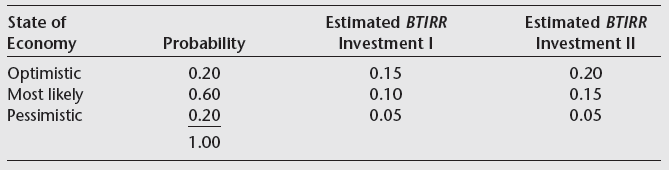
\includegraphics[width=300 px]{p2_447} \end{center}

Riskless is aware that the pattern of returns for Investment II looks
very attractive relative to Investment I; however, he believes that
Investment II could be more risky than Investment I. He would like to
know how he can compare the two investments considering both the risk
and return on each. What do you suggest?

\end{frame}

\begin{frame}[fragile]{Problem 2 (p.447) Answers}

\begin{Shaded}
\begin{Highlighting}[]
\CommentTok{# See excel}
\end{Highlighting}
\end{Shaded}

\end{frame}

\begin{frame}{Exercise: Real option approach}

\footnotesize

A land owner is trying to decide whether to develop her land. She
expects the market to perform at worst and at best as follows:

\begin{longtable}[]{@{}llllll@{}}
\toprule
Scenario & price & units & costs & Rent (year) & Interest\tabularnewline
\midrule
\endhead
Current & 220K & 10 & 110K & 8k & 5\%\tabularnewline
Optimistic & 250K & 15 & 120K & 8k & 5\%\tabularnewline
Pessimistic & 220K & 10 & 110K & 8k & 5\%\tabularnewline
\bottomrule
\end{longtable}

\begin{enumerate}
\def\labelenumi{\arabic{enumi}.}
\tightlist
\item
  Calculate the value of land today.
\item
  calculate the value of the land conditional on realization of each of
  the two scenarios.
\item
  Follow the real option approach to calculate the \(\alpha\) and
  \(\beta\) values of the replicate portfolio, assuming no construction.
  Keep in mind to consider rent payment returns, and interest paid for
  the risk-free assets in the replicate potfolio.
\item
  Calculate the value of the replicate portfolio. What would be the
  optimal strategy that the developer should follow?
\end{enumerate}

\normalsize

\end{frame}

\begin{frame}[fragile]{Exercise: Real option approach}

\begin{Shaded}
\begin{Highlighting}[]
\CommentTok{# See excel}
\end{Highlighting}
\end{Shaded}

\end{frame}

\begin{frame}{Problem 1 (p.482)}

\small

A property could be sold today for \$2 million. It has a loan balance of
\$1 million and, if sold, the investor would incur a capital gains tax
of \$250,000.

The investor has determined that if it were sold today, she would earn
an IRR of 15\% on equity for the past five years. If not sold, the
property is expected to produce after-tax cash flow of \$50,000 over the
next year.

At the end of the year, the property value is expected to increase to
\$2.1 million, the loan balance will decrease to \$900,000, and the
amount of capital gains tax due is expected to increase to \$255,000.

\begin{enumerate}
\def\labelenumi{\arabic{enumi}.}
\tightlist
\item
  What is the marginal rate of return for keeping the property one
  additional year?
\item
  What advice would you give the investor?
\end{enumerate}

\end{frame}

\begin{frame}[fragile]{Problem 1 (p.482) Answers}

\footnotesize

\begin{center}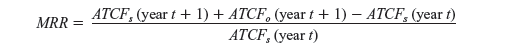
\includegraphics[width=300 px]{mrr} \end{center}

\begin{Shaded}
\begin{Highlighting}[]
\CommentTok{# 1 }
\NormalTok{ATCFs =}\StringTok{ }\NormalTok{(sale price -}\StringTok{ }\NormalTok{mortgage value -}\StringTok{ }\NormalTok{capital gain tax)}
\KeywordTok{ATCFs} \NormalTok{(today) =}\StringTok{ }\NormalTok{(}\DecValTok{2000000} \NormalTok{-}\StringTok{ }\DecValTok{1000000} \NormalTok{-}\StringTok{ }\DecValTok{250000}\NormalTok{) =}\StringTok{ }\DecValTok{750000}
\KeywordTok{ATCFs} \NormalTok{(+1Y) =}\StringTok{ }\NormalTok{(}\DecValTok{2100000} \NormalTok{-}\StringTok{ }\DecValTok{900000} \NormalTok{-}\StringTok{ }\DecValTok{255000}\NormalTok{) =}\StringTok{ }\DecValTok{945000}
\KeywordTok{ATCFo} \NormalTok{(+1Y) =}\StringTok{ }\DecValTok{50000}

\NormalTok{MRR =}\StringTok{ }
\NormalTok{(}\DecValTok{945000} \NormalTok{-}\StringTok{ }\DecValTok{750000} \NormalTok{+}\StringTok{ }\DecValTok{50000}\NormalTok{)/}\DecValTok{750000} \NormalTok{=}\StringTok{ }\FloatTok{0.3266}
\end{Highlighting}
\end{Shaded}

\end{frame}

\begin{frame}{Problem 2 (p.482)}

\small

The owner (from previous problem) determines that if the property were
renovated instead of sold, after-tax cash flow over the next year would
increase to \$60,000 and the property could be sold after one year for
\$2.4 million. Renovation would cost \$250,000. The investor would not
borrow any additional funds to renovate the property.

\begin{enumerate}
\def\labelenumi{\arabic{enumi}.}
\tightlist
\item
  What is the rate of return that the investor would earn on the
  additional funds invested in renovating the property?
\item
  Would you recommend that the property be renovated?
\end{enumerate}

\end{frame}

\begin{frame}[fragile]{Problem 2 (p.482) Answers}

\footnotesize

\begin{Shaded}
\begin{Highlighting}[]
\CommentTok{# 1 }

\NormalTok{d }\KeywordTok{ATCFs} \NormalTok{(+1Y) =}\StringTok{ }\NormalTok{Additional sale revenue -}\StringTok{ }\NormalTok{Revonvation costs}
  \NormalTok{=}\StringTok{ }\NormalTok{(}\DecValTok{2400000} \NormalTok{-}\StringTok{ }\DecValTok{2100000}\NormalTok{) -}\StringTok{ }\NormalTok{(}\DecValTok{250000}\NormalTok{) =}\StringTok{ }\DecValTok{50000}
  
\NormalTok{d }\KeywordTok{ATCFo} \NormalTok{(+1Y) =}\StringTok{ }\NormalTok{Difference in cash flow }
  \NormalTok{(}\DecValTok{60000-50000}\NormalTok{) =}\StringTok{ }\DecValTok{10000}

\NormalTok{MRR =}\StringTok{ }
\NormalTok{(}\DecValTok{50000} \NormalTok{+}\StringTok{ }\DecValTok{10000}\NormalTok{)/}\DecValTok{250000} \NormalTok{=}\StringTok{ }\FloatTok{0.24}
\end{Highlighting}
\end{Shaded}

\normalsize

\end{frame}

\end{document}
